\chapter{提案手法}

\section{象の卵の大きさ}
外形を計測し,それが絶対的な卵の形の枠であるアルキメデスの円筒座標表示形(式(\ref{Archimedes}))と一致するかどうか調べる。もし一致していなければ、卵でない可能性がある。
\subsection{サブセクションのテスト}
\subsubsection{サブサブセクションのテスト}
%%
%% 以下,番号つきディスプレイ数式モードの例
%%
\begin{equation}
r(z)=0.5\sqrt{1-(e^z-2)^2}
\label{Archimedes}
\end{equation}
%%
%% inline数式モードの例
%%
ここで,$r$は$z$軸からの距離,$z$は$xy$に直行する軸方向で,直交座標系は右手座標系であるとする。すなわち,$\hat{\bm{x}}$,$\hat{\bm{y}}$,$\hat{\bm{z}}$を,それぞれ$x$,$y$,$z$軸方向の単位ベクトルとしたとき,$\hat{\bm{z}} = \hat{\bm{x}} \times \hat{\bm{y}}$が成立している。
また,$r$の偏微分$\frac{\partial r}{\partial z}$は...
%%
%% 式番をまとめて表示する例
%%

ところで,カモメ(図\ref{kamome})が$x$羽,象が$y$匹としたときに,頭の数と,足の数の関係から,
\begin{eqnarray}
  \begin{cases}
    x + y = 2 & \\
    2x + 4y = 6 &
  \end{cases}
\end{eqnarray}

%%
%% 図の入れ方の例
%%
\begin{figure}[tb]
  \begin{center}
   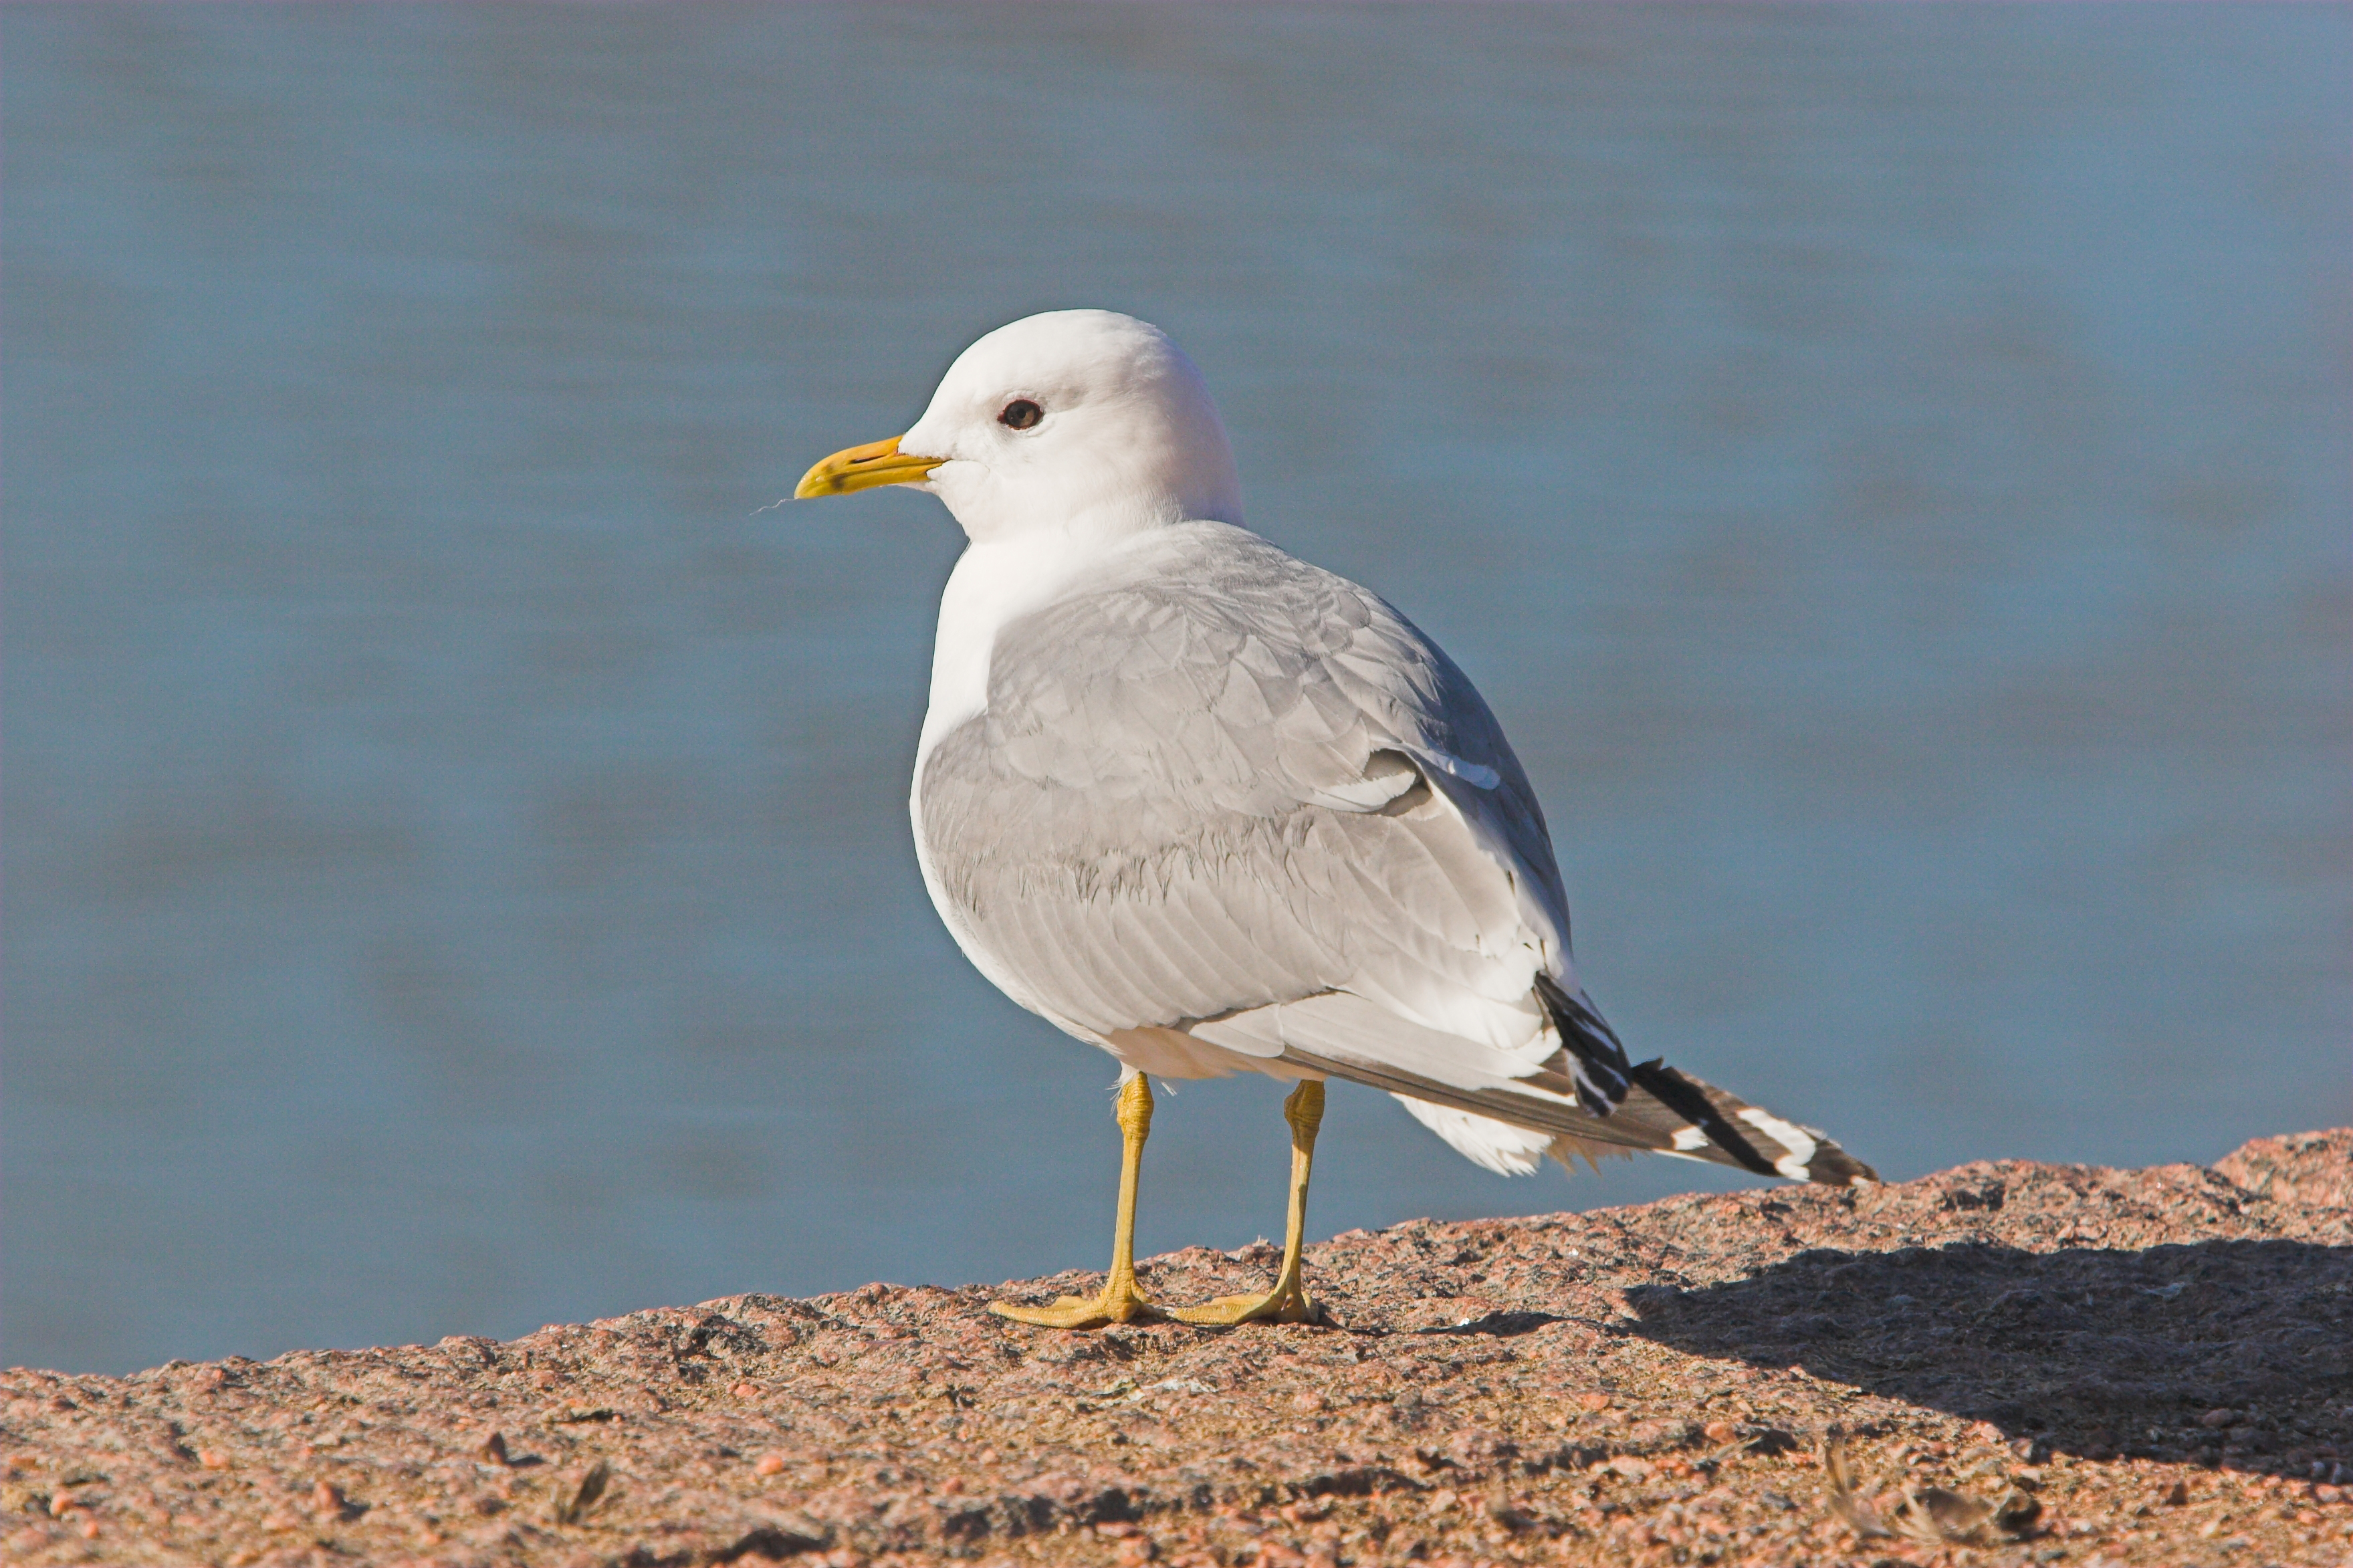
\includegraphics[width=0.4\linewidth]{image/kamome.jpg}
  \end{center}
  \caption{カモメ}
  \label{kamome}
\end{figure}
